\documentclass[12pt,fleqn]{article}\usepackage{../common}
\begin{document}
Rasgele �zd���m� (Random Projection) ile SVD

Eger ana matrisimiz $A$'nin cok fazla kolonu var ise bunu bir sekilde
azaltmanin yollarini arayabiliriz. [1]'e gore bunu yapmanin
yollarindan biri rasgele izdusum hesabidir. Ilk once $n \times k$
boyutunda bir Gaussian rasgele matris $\Omega$ uretiriz. Ardindan

$$ Y = A\Omega $$

hesaplanir. Bu $Y$ uzerinde QR ayristirmasi yapariz, ve elde edilen $Q$ ile

$$ B = Q^T A $$

hesabini yapariz. Ardindan bu matris uzerinde SVD ayristirmasi yapariz,

$$ B = \hat{U}\Sigma V^T $$

ve

$$ U = Q\hat{U} $$

matrisini hesaplariz. Ana fikir suradan geliyor,

$$ A = QQ^TA $$

ki bu standart bir cebir numarasi olurdu, $Q$ yerine rasgele
izdusumdan gelen yaklasiksal $Q$'yu kullanabiliriz, o zaman

$$ A \approx \tilde{Q}\tilde{Q}^TA $$

olacaktir. Yani izdusumden gelen $Q,R$ gercek versiyona yakin. Ustteki
carpimda $R$ yerine $B$ harfi kullaniyoruz, ki $B = \tilde{Q}^T A$
oluyor, yani

$$ A \approx \tilde{Q}B $$

ya da 

$$ B \approx \tilde{Q}^T A $$.

O zaman Istatistik notlarimiz altindaki *Paralel Matris Carp�m�, Ax,
QR ve SVD* yazisinda oldugu gibi $B$'nin SVD'sini alarak yaklasiksal
bir $U$ elde etmek mumkun olacaktir.

Bu yaklasiksal metot isler cunku noktalari yaklasiksal bir altuzaya
yansittiktan sonra elde edilen yeni noktalarin arasindaki mesafelerin
fazla bozulmadan muhafaza edildigi soylenir, daha detayli soylemek
gerekirse, n-boyutlu verileri $O(\log n / \epsilon^2)$ boyutundaki bir
rasgele altuzaya yansitmak, pozitif olasilikla, yeni noktalarin
arasindaki mesafeleri sadece $1 \pm \epsilon$ olcusunde degistirir
[2]. $Y$'nin, $A$'nin "menzilini" iyi temsil ettigi de soylenir.

Test olarak suradaki [3] veri seti uzerinde gorelim:

\begin{minted}{python}
import numpy.random as rand
import numpy.linalg as lin
import pandas as pd

k = 7 # izdusum uzayinin boyutlari
df = pd.read_csv("w1.dat",sep=';',header=None)
A = np.array(df)[:,1:]

print "A",A.shape

rand.seed(1000)

Omega = rand.randn(A.shape[1],k)

Y = np.dot(A, Omega) 

print "Y", Y.shape

Q, R = lin.qr(Y) 

# niye devrigi ile is yaptigimizi altta anlatiyoruz
BT = np.dot(A.T, Q)

print "Q", Q.shape
print "BT", BT.shape

x, x, V = lin.svd(BT)

print 'V', V.shape

Uhat = V.T # cunku B=USV', B'=VSU' U of B icin V' lazim

print "Uhat", Uhat.shape

U = np.dot(Q, Uhat) 

print "U", U.shape

plt.plot(U[:,0],U[:,1],'r+')

plt.hold(True)
        
# gercek SVD ile karsilastir

U, Sigma, V = lin.svd(A);
plt.plot(U[:,0],-U[:,1],'bx')
plt.savefig('rnd_1.png')
\end{minted}

\begin{verbatim}
A (71, 30)
Y (71, 7)
Q (71, 7)
BT (30, 7)
V (7, 7)
Uhat (7, 7)
U (71, 7)
\end{verbatim}

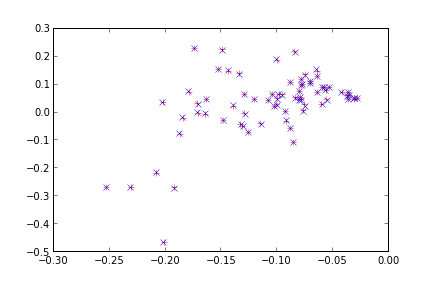
\includegraphics[height=6cm]{rnd_1.png}

Mavi noktalar $A$ uzerinde "gercek" SVD sonucu, kirmizilar yansitma
sonrasi elde edilen $U$. Sonuclar cok iyi. 

$B$ yerine $B^T$

Kodlama acisindan, ya da buyuk veri baglaminda baska amaclar [4] icin
$B = Q^T A$ yerine $B^T = A^T Q$ hesabi yapmak istenilebilir. Niye?
Cunku cikti olarak $n \times k$ matrisi istiyor olabiliriz, $k \times
n$ matrisi istemiyoruz, yani cok olanin satirlar olmasini istiyoruz,
kolonlar olmasini istemiyoruz.

O zaman, elde edilen $B^T$ ise, $B$ uzerinde degil $B^T$ uzerinde SVD
alacagiz demektir, bu da sonuclari birazcik degistirir, yani

$$ B = U\Sigma V^T $$

$$ B^T = V\Sigma U^T $$

haline gelir. Yani $B$'nin $U$'sunu elde etmek icin $B^T$'nin SVD'si
sonrasinda ele gecen sonucta $(U_{BT}^T)^T$ yapmak gerekir. Her seyin
hafizada yapildigi durumda bu fark yaratmaz, fakat "ilerisi icin", yani
esle / indirge ortamlari icin akilda tutmak faydali olur.

Kaynaklar

[1] Halko, N., Randomized methods for computing low-rank
approximations of matrices

[2] Gupta, A., Dasgupta, S., An Elementary Proof of a Theorem of Johnson and Lindenstrauss

[3] \verb!archive.ics.uci.edu/ml/datasets/Breast+Cancer!

[4] \verb!arxiv.org/abs/1310.4664!


\end{document}
